\section{Content of enclosed CD}
\label{appendix:cd-contents}


    \begin{enumerate}
    \item /docs/
    \item /pdsurvey/
    \item /pdemail/
    \item /pdclient-static/
    \item Google Docs
    \end{enumerate}



%% - - -  D O C U M E N T A T I O N  - - - %%

\section{Documentation of Platform}
\label{appendix:documentation}

  A user, developer and maintenance documentation for the PDSurvey platform can be found in the GitHub repository \footnote{https://github.com/lukasziegler/masterarbeit/tree/master/docs} and on the enclosed CD.



%% - - - -  P A P E R S   R E A D  - - - - %%

\section{Papers Evaluating Public Displays}
  
  List of relevant papers, which include an evaluation of public displays.

  TABLE: 1st column (paper), 2nd column evaluation (quantitative, qualitative, no evaluation)

  TODO



%% - - - Q U E S T I O N N A I R E S - - - %%

\section{Questionnaires used for Evaluation}
\label{appendix:papers}

  Embed the following PDFs

  \begin{enumerate}
  \item interview-participants.pdf \label{appendix:interview-participant}
  \item interview-passerby.pdf \label{appendix:interview-passerby}
  \item semi-structured-interview.pdf \label{appendix:semi-structured-interview}
  \end{enumerate}



%% - - - - S C R E E N S H O T S - - - - %%

\section{Screenshots of Platform}
\label{appendix:screenshots-balloon-shooter}

    All screenshots including the copyright of the Balloon Shooter game belong to Jiamin Shi. 
    
    \begin{figure}
        \begin{center}
            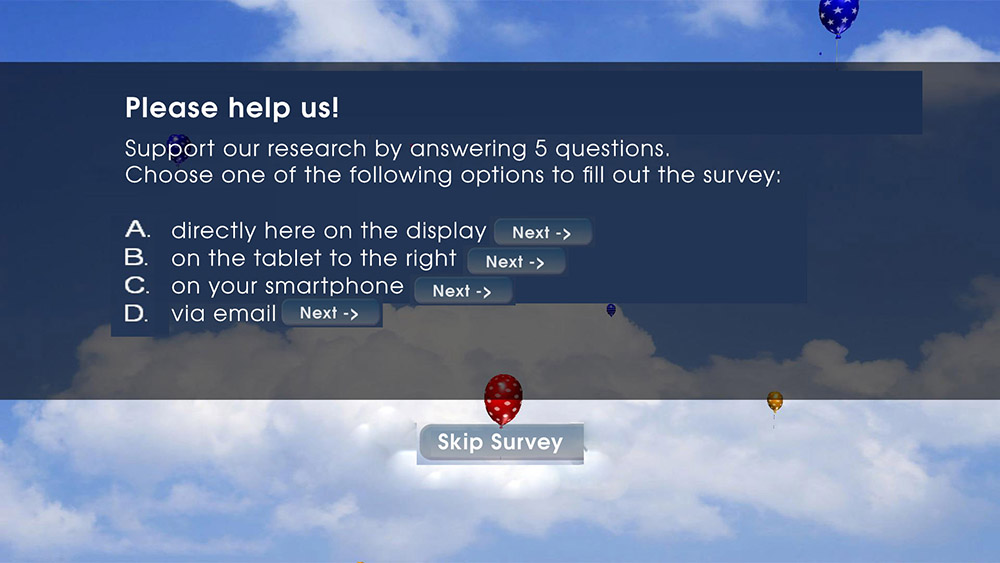
\includegraphics[width=\columnwidth]{img/screenshots/options-overview.jpg}
        \end{center}
     \caption{All four four options for completing a survey, the order being randomized on every instance.}
     \label{screenshot:options}
    \end{figure}


    1st option: tv screen

    \begin{figure}
        \begin{center}
            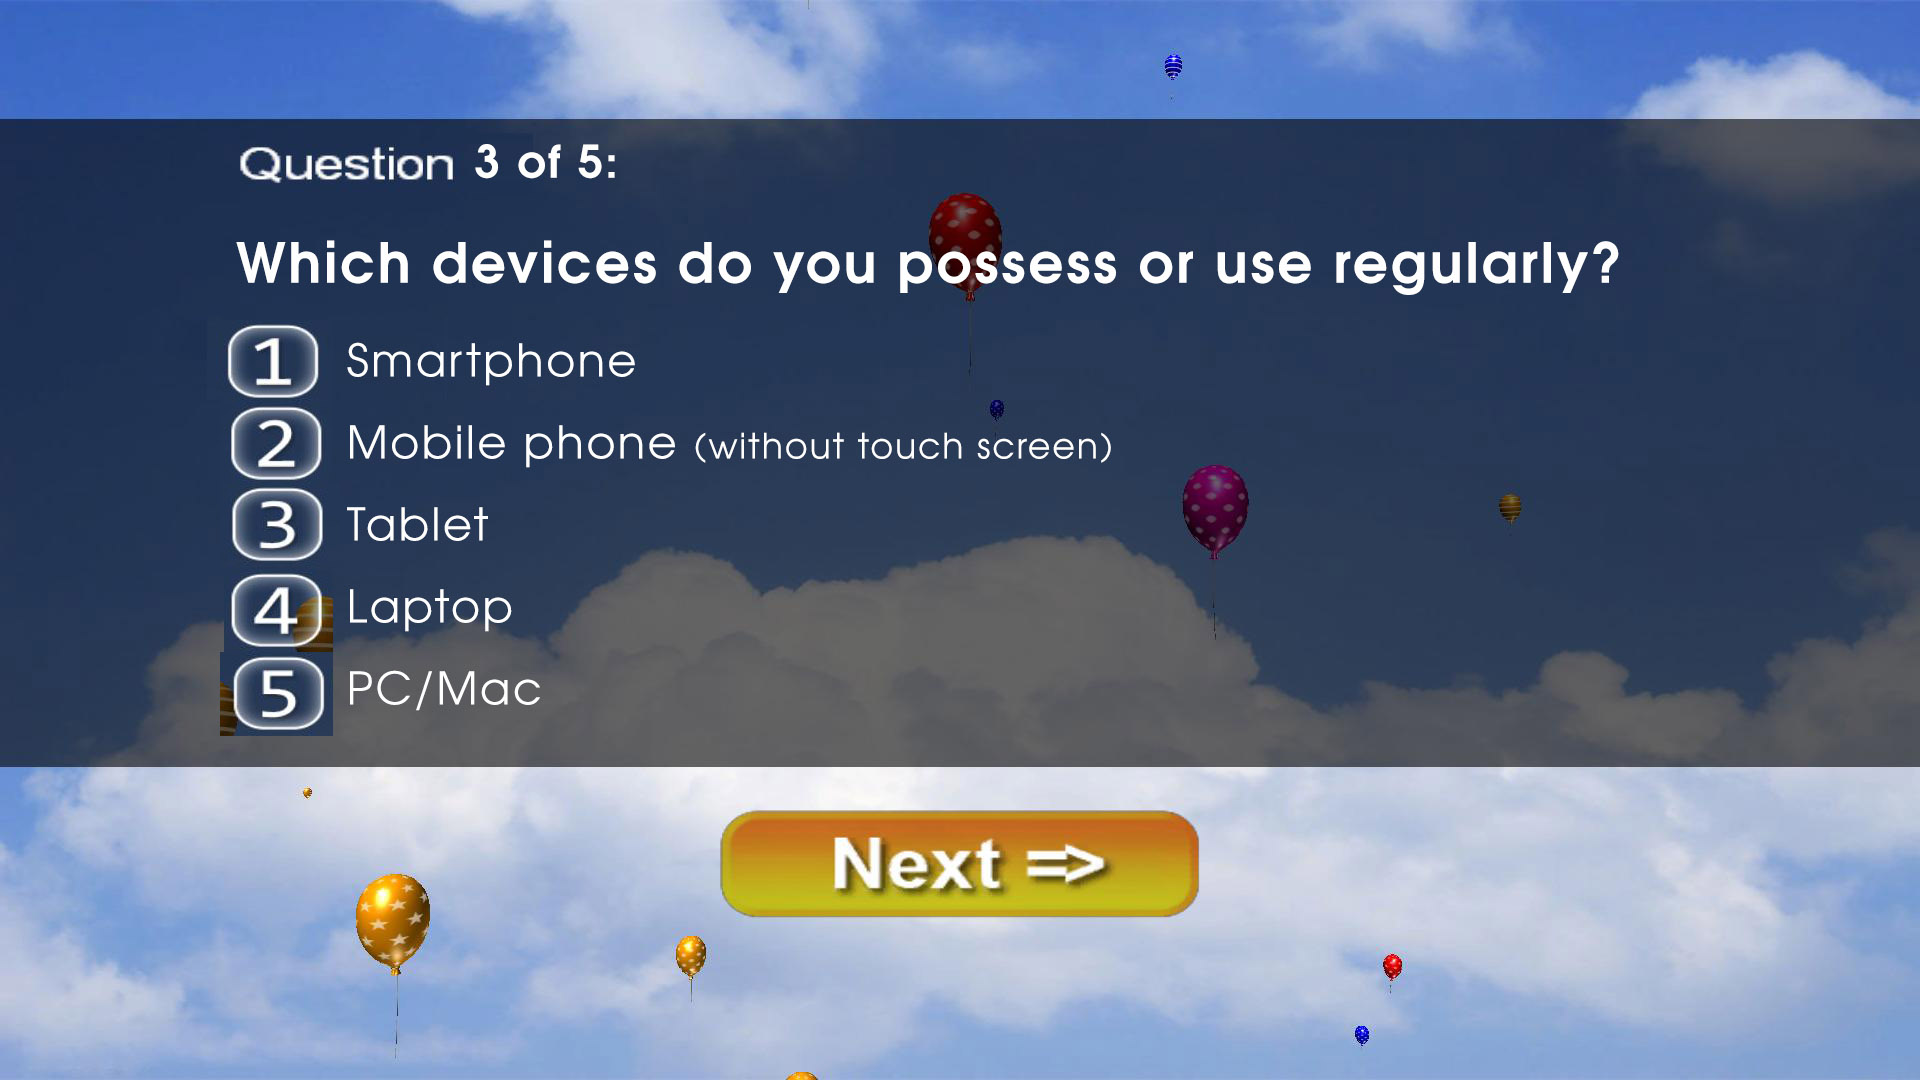
\includegraphics[width=\columnwidth]{img/screenshots/option-tv.jpg}
        \end{center}
     \caption{Option 1, directly answering on the TV screen. Here you see a sample question getting asked on the interactive display.}
     \label{screenshot:tv-option}
    \end{figure}


    2nd option: tablet

    \begin{figure}
        \begin{center}
            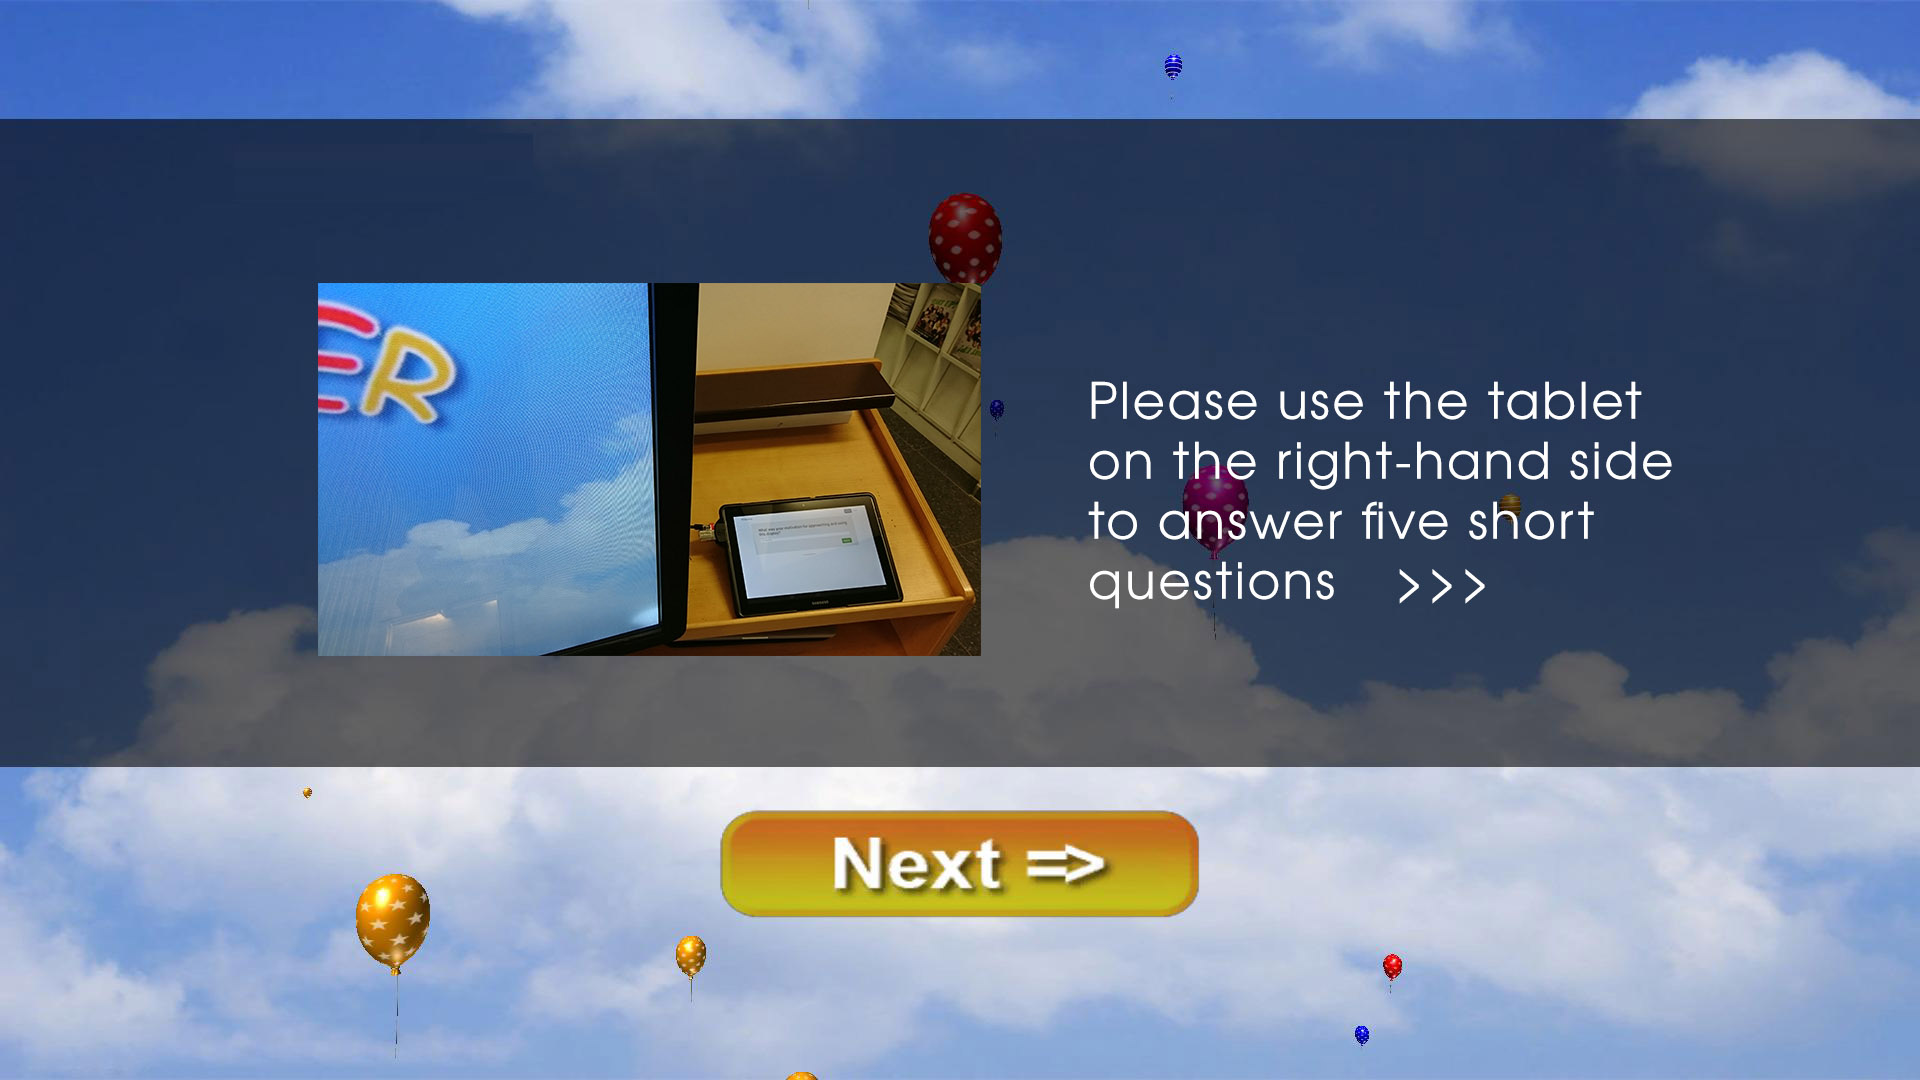
\includegraphics[width=\columnwidth]{img/screenshots/option-tablet.jpg}
        \end{center}
     \caption{Option 2, the screen the user sees when choosing to complete the survey on the tablet.}
     \label{screenshot:tablet-option}
    \end{figure}


    3rd option: smartphone

    \begin{figure}
        \begin{center}
            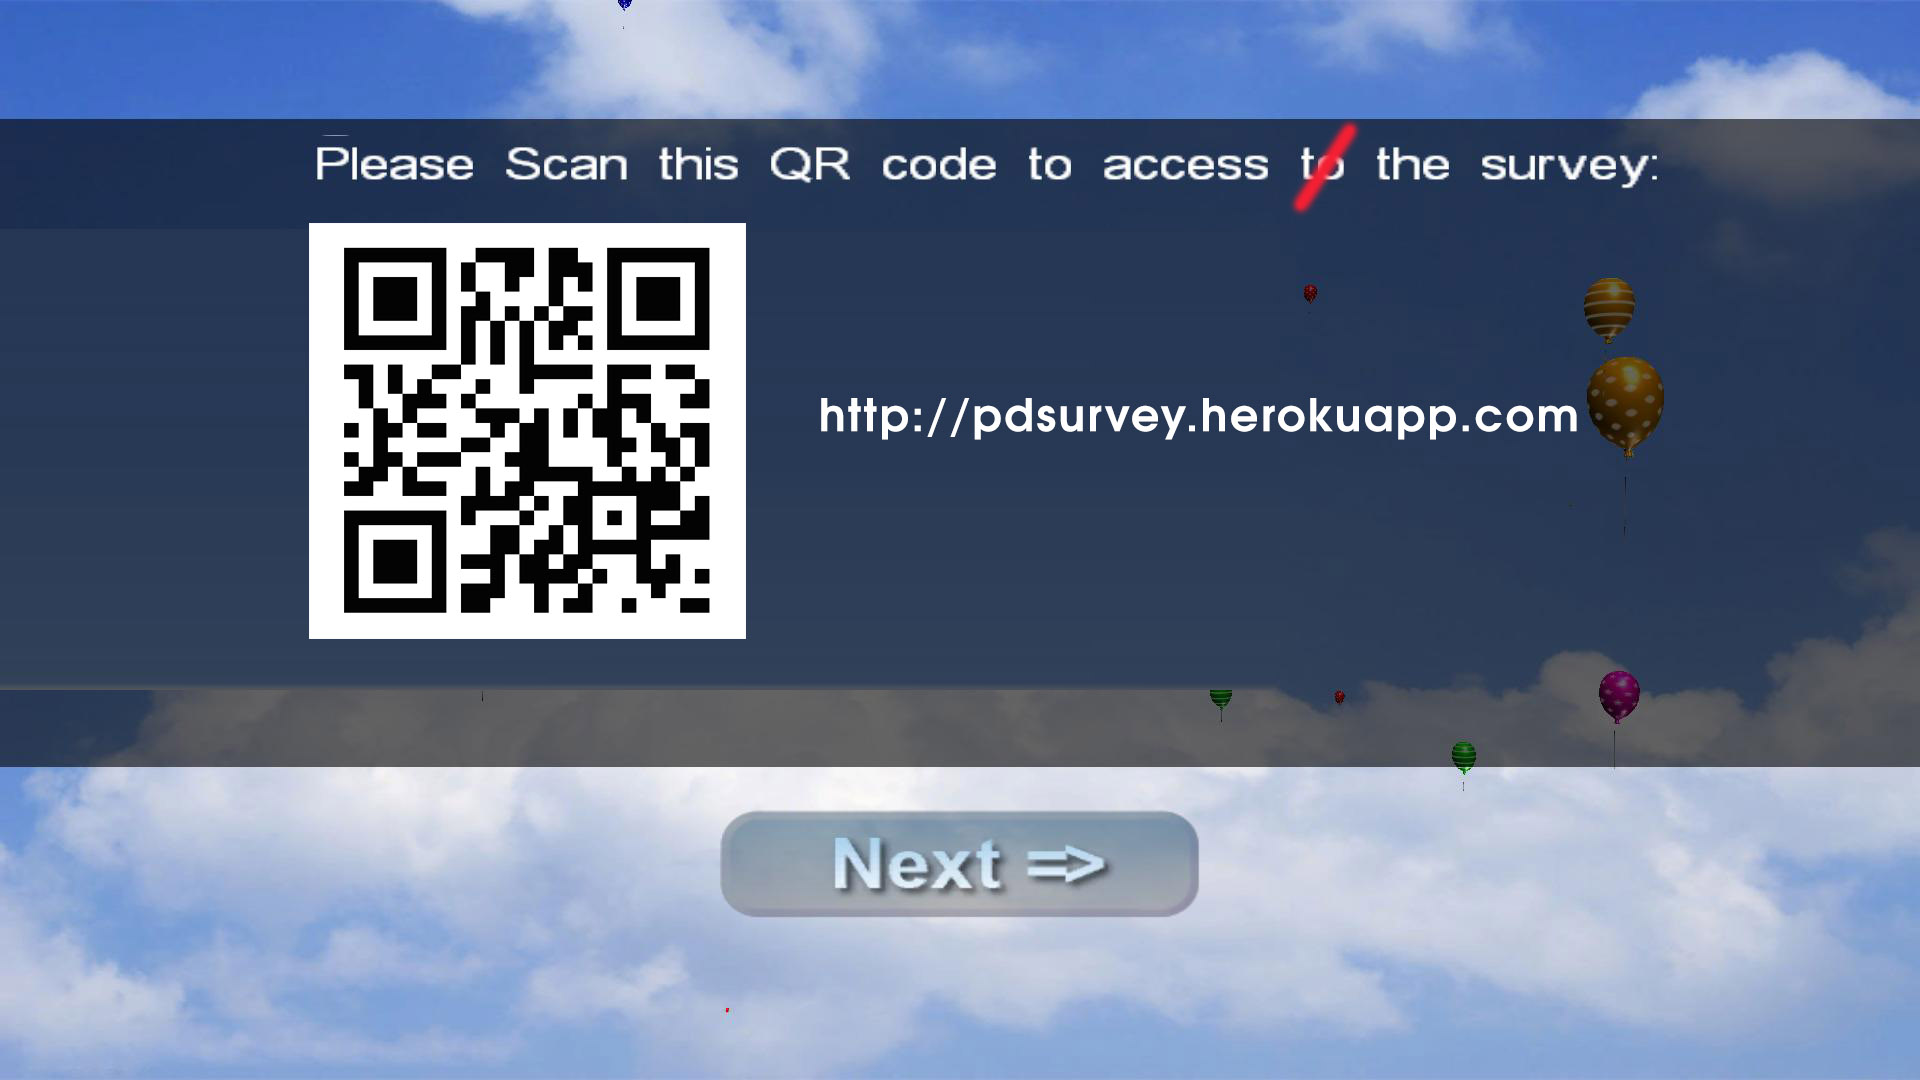
\includegraphics[width=\columnwidth]{img/screenshots/option-smartphone.jpg}
        \end{center}
     \caption{Option 3, participating with your own smartphone, either by scanning the QR code or by typing the URL in the mobile browser.}
     \label{screenshot:smartphone-option}
    \end{figure}


    4th option: email

    \begin{figure}
        \begin{center}
            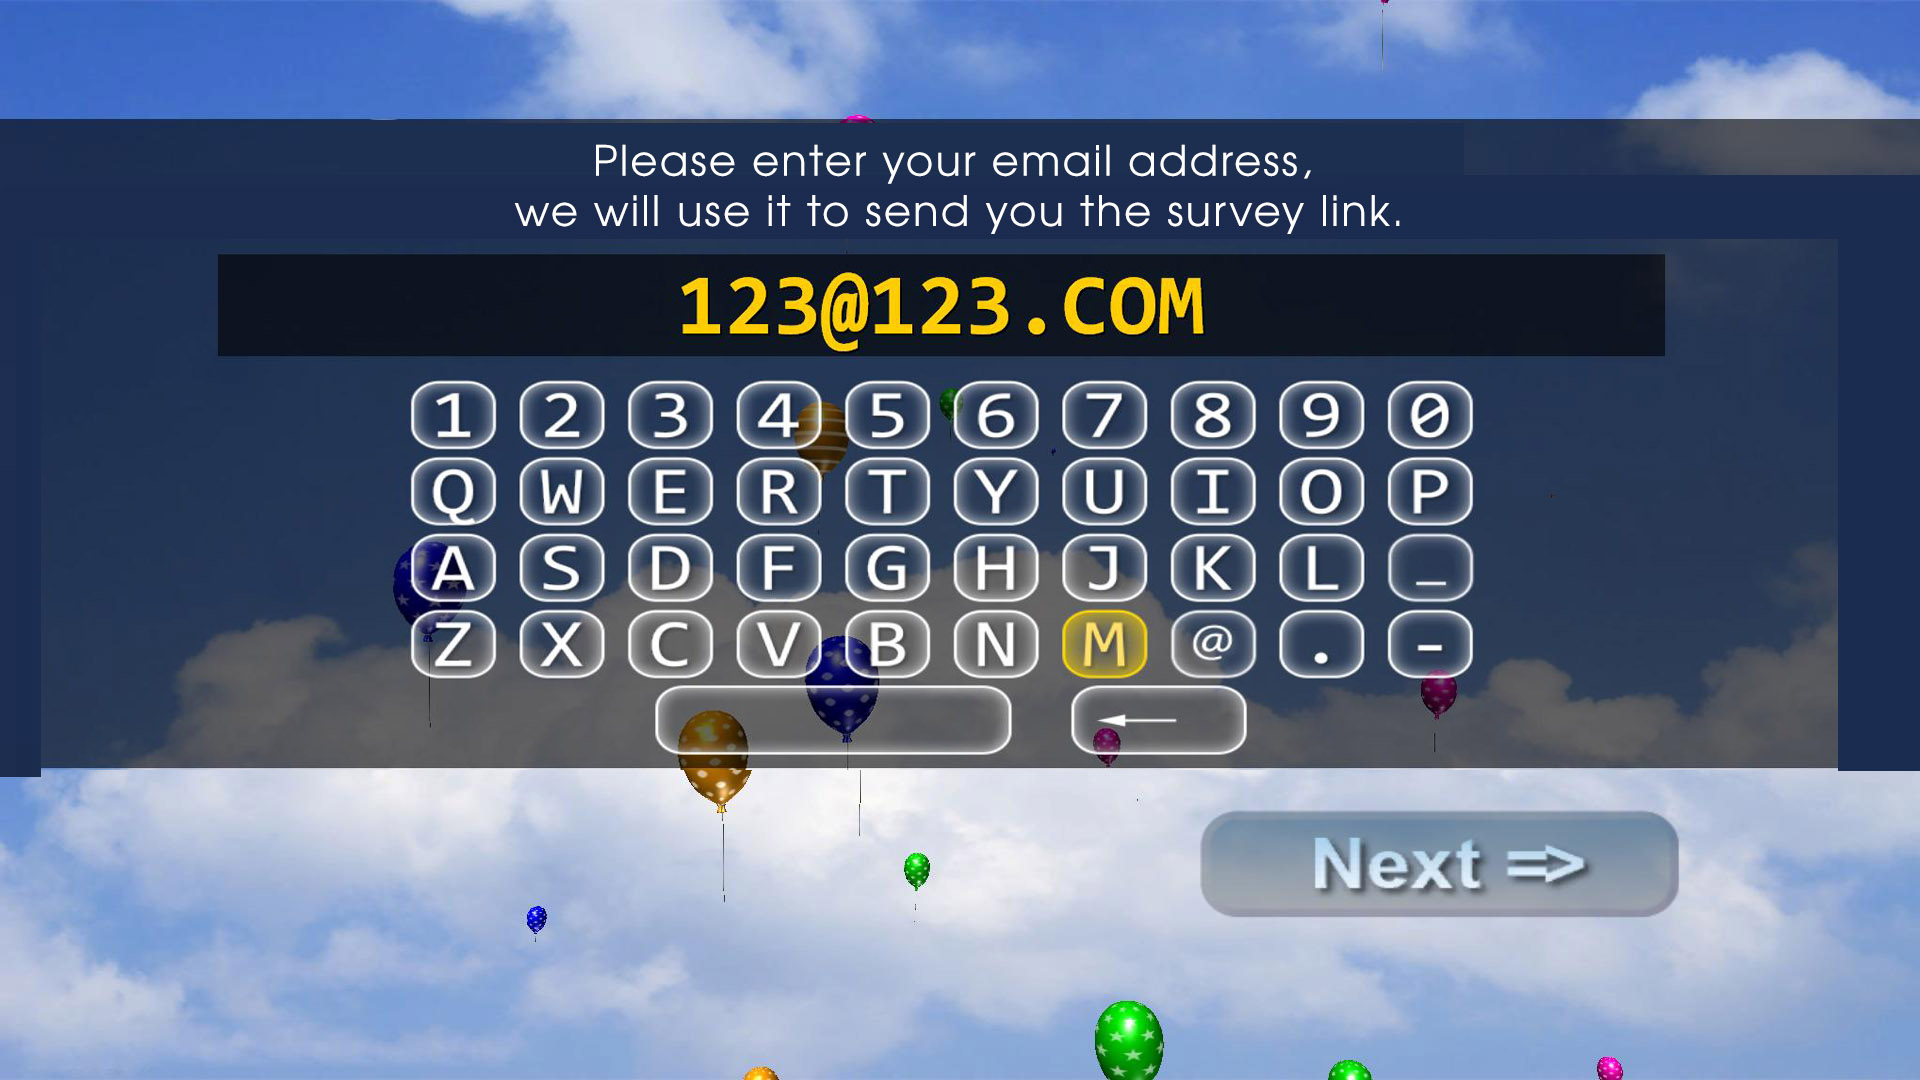
\includegraphics[width=\columnwidth]{img/screenshots/option-email.jpg}
        \end{center}
     \caption{Option 4, submitting ones email address and getting the survey link to participate in response.}
     \label{screenshot:email-option}
    \end{figure}